\subsection{Problem 31: Vectors and Ratios}

\begin{problem}
The point $C$ divides the interval $AB$ so that $\frac{CB}{AC} = \frac{m}{n}$. The position vectors of $A$ and $B$ are $\mathbf{a}$ and $\mathbf{b}$ respectively, as shown in the diagram below.

\vspace{0.5em}
\noindent
\begin{center}
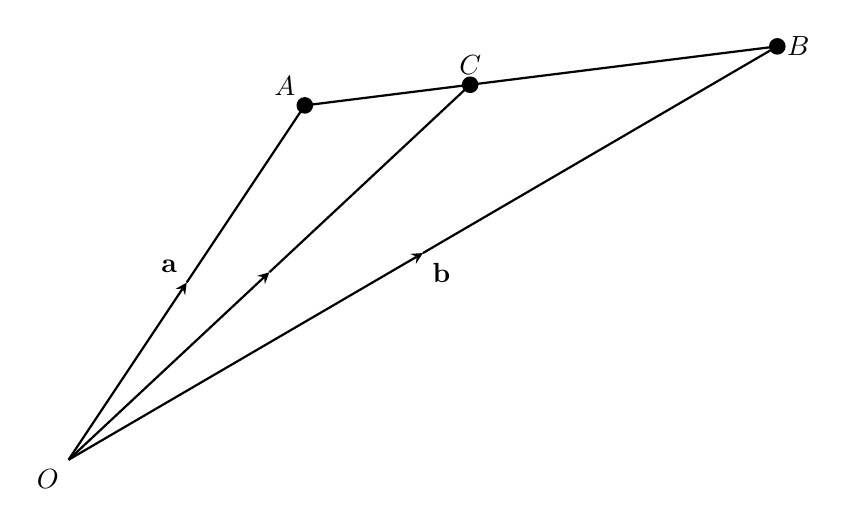
\begin{tikzpicture}[scale=1.5, >=stealth]
    % Coordinates of the points
    \coordinate (O) at (0,0);
    \coordinate (A) at (2,3);
    \coordinate (B) at (6,3.5);
    \coordinate (C) at (3.4, 3.175);
    
    % Midpoints for vector arrows
    \coordinate (midA) at (1, 1.5);
    \coordinate (midB) at (3, 1.75);
    \coordinate (midC) at (1.7, 1.5875);
    
    % Draw vector OA with arrow in the middle
    \draw[->, thick] (O) -- (midA);
    \draw[thick] (midA) -- (A);
    
    % Draw vector OB with arrow in the middle
    \draw[->, thick] (O) -- (midB);
    \draw[thick] (midB) -- (B);
    
    % Draw vector OC with arrow in the middle
    \draw[->, thick] (O) -- (midC);
    \draw[thick] (midC) -- (C);
    
    % Draw line segment AB
    \draw[thick] (A) -- (B);
    
    % Draw dots at A, B, C
    \fill (A) circle (2pt);
    \fill (B) circle (2pt);
    \fill (C) circle (2pt);
    
    % Point labels
    \node[below left] at (O) {$O$};
    \node[above left] at (A) {$A$};
    \node[right] at (B) {$B$};
    \node[above] at (C) {$C$};
    
    % Vector labels
    \node[above left] at (midA) {$\mathbf{a}$};
    \node[below right] at (midB) {$\mathbf{b}$};
\end{tikzpicture}
\end{center}
\vspace{0.3em}

\begin{enumerate}
    \item[(i)] Show that $\vec{AC} = \frac{n}{m+n}(\mathbf{b} - \mathbf{a})$.
    
    \item[(ii)] Prove that $\vec{OC} = \frac{m}{m+n}\mathbf{a} + \frac{n}{m+n}\mathbf{b}$.
\end{enumerate}
\end{problem}

\begin{hint}
For part (i), use the ratio $\frac{CB}{AC} = \frac{m}{n}$ and the fact that $AC + CB = AB$. For part (ii), use $\vec{OC} = \vec{OA} + \vec{AC}$.
\end{hint}

